\section{Электродвигатель}

\subsection{Устройство двигателя постоянного тока}

\begin{figure}[h]
\centering
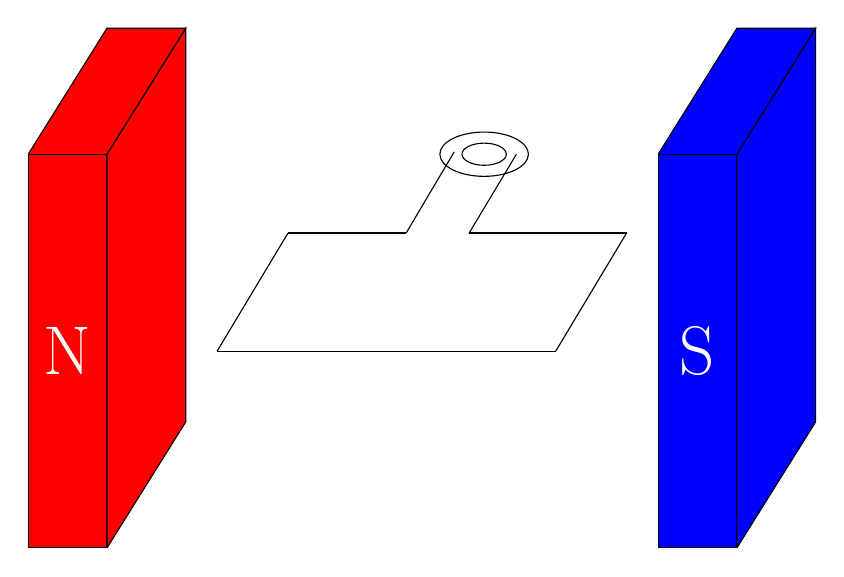
\begin{tikzpicture}

%красный полюс

\draw[fill=red] (0,0) rectangle (1,5);
\draw[fill = red] (1,0) --  (2,1.6) -- (2,6.6) -- (1,5) -- (1,0); 
\draw[fill = red]  (0,5) -- (1,6.6) -- (2,6.6) -- (1,5);
\draw[white] (0.5,2.5) node {\Huge{N}} (1,2.5);
\draw (0,5) -- (1,5);

%синий полюс
\draw[fill=blue] (8,0) rectangle (9,5);
\draw[fill = blue] (9,0) --  (10,1.6) -- (10,6.6) -- (9,5) -- (9,0); 
\draw[fill = blue]  (8,5) -- (9,6.6) -- (10,6.6) -- (9,5);
\draw[white] (8.5,2.5) node {\Huge{S}} (9,2.5);
\draw (8,5) -- (9,5);

%рамка
\draw (2.4,2.5) -- (6.7,2.5); %ближнаяя горизонтальная
\draw (2.4,2.5) -- (3.3,4); % левая
\draw (3.3,4) -- (4.8,4); \draw (5.6,4) -- (7.6,4); %верхняя слева + справа
\draw (6.7,2.5) -- (7.6,4); % правая
\draw (4.8,4) -- (5.41,5.03); \draw (5.6,4) -- (6.2,5); % контакты

%переход на цепь

\draw (5.79,5) ellipse [x radius=8pt, y radius=4pt];
\draw (5.79,5) ellipse [x radius=16pt, y radius=8pt];

%\draw (5.8,5) circle [radius=0.5];
%\draw (5.8,5) circle [radius=0.3];

\end{tikzpicture}
\caption{Принцип работы электродвигателя}
\label{fig:electro_engine}

\end{figure}

\subsection{Изменение направления и скорости вращения двигателя}

\begin{enumerate}
    \itemСоберите по очереди схемы, представленные на рисунке \ref{fig:7.1}. Укажите в каждом случае направление силы тока при зажатой кнопке К.
    \itemДля каждой схемы выполните следующее занятие:
    \begin{enumerate}
        \itemУстановите пропеллер на двигатель. Зажмите кнопку К и наблюдайте за направлением и частотой вращения пропеллера.\label{7.1}
        \itemРазверните двигатель на 180°и повторите пункт \ref{7.1}.
    \end{enumerate}
    \itemСделайте вывод о зависимости частоты вращения двигателя от приложенного напряжения и о зависимости направления вращения двигателя от направления тока. Запишите выводы. 

\begin{figure}[h]
\begin{minipage}[h]{0.5\linewidth}
\center{\begin{circuitikz} 
\draw
(0,0) to[battery, invert] (0,4)to[Telmech=M](4,4) -- (4,0) to[push button, mirror, a=$K$] (0,0)
;
\end{circuitikz}\\ а.}
\end{minipage}
\hfill
\begin{minipage}[h]{0.5\linewidth}
\center{\begin{circuitikz} \draw
(0,0) to[battery, invert] (0,4)to[Telmech=M](4,4) to[battery, invert] (4,0) to[push button, mirror, a=$K$] (0,0)
;
\end{circuitikz} \\ б.}
\end{minipage}
\caption{Изменение направления и скорости двигателя}
\label{fig:7.1}
\end{figure}



Вывод --- \hrulefill

\hrulefill

\hrulefill

\end{enumerate}

\subsection{Электродвигатель в качестве генератора}

\begin{enumerate}
    \itemСоберите схему, представленную на рисунке \ref{fig:7.2}.
    \itemВращайте вал двигателя по/против часовой стрелки с различной частотой и наблюдайте за показаниями вольтметра.
    \itemЗапишите выводы о возможности применения электродвигателя в качестве генератора, о зависимости полярности создаваемого ЭДС от направления вращения двигателя, а также о зависимости величины создаваемого ЭДС от скорости вращения двигателя.
\end{enumerate}

\begin{figure}[h]
\centering
\begin{circuitikz} 
\draw
(0,0) -- (0,2)to[Telmech=M](4,2) -- (4,0) to[rmeter, t=$V$] (0,0)
;
\end{circuitikz}
\caption{Электродвигатель в качестве генератора}
\label{fig:7.2}
\end{figure}

Вывод --- \hrulefill

\hrulefill

\hrulefill

\subsection{Регулирование частоты вращения двигателя и реверс двигателя}

\begin{enumerate}
    \itemСоберите схему, представленную на рисунке \ref{fig:7.3}. Укажите направление силы тока в цепи при верхнем/среднем/нижнем положении движка реостата. 
    \itemЗамкните выключатель К. Перемещая движок реостата, наблюдайте за направлением и скоростью вращения электродвигателя.
    \itemЗапишите выводы о возможности регулирования направления и частоты вращения двигателя.
\end{enumerate}

\begin{figure}[h]
\centering
\begin{circuitikz} 
\draw (4,4) to[pR, name=R, mirror] (4,0);
\draw (0,0)to[battery1, invert] (0,1)to[battery1, invert](0,2)to[battery1, invert](0,3) to[battery1, invert](0,4);
\draw (0,2) to[normal open switch, l=$K$] (2,2)to[Telmech=M] (R.wiper);
\draw (0,4) -- (4,4);
\draw (0,0) -- (4,0);
\end{circuitikz}
\caption{Регулирование частоты вращения двигателя и реверс двигателя}
\label{fig:7.3}
\end{figure}

Вывод --- \hrulefill

\hrulefill

\hrulefill


\subsection{Пуск двигателя}

\begin{enumerate}
    \itemСоберите схему, представленную на рисунке \ref{fig:7.4}. Укажите направление силы тока в ней при зажатой кнопке К.
    \itemЗажмите кнопку К и наблюдайте за яркостью свечения лампы. Аккуратно и кратковременно (на одну секунду) затормозите вращение двигателя и наблюдайте за яркостью свечения лампы.
    \itemЗапишите выводы о зависимости яркости свечения лампы от частоты вращения двигателя.
\end{enumerate}

\begin{figure}[h]
\centering
\begin{circuitikz} 
\draw
(0,0) to[battery, invert] (0,4)to[Telmech=M](4,4) to[lamp] (4,0) to[push button, mirror, a=$K$] (0,0)
;
\end{circuitikz}
\caption{Пуск двигателя}
\label{fig:7.4}
\end{figure}

Вывод --- \hrulefill

\hrulefill

\hrulefill

\newpage